\documentclass[12pt]{article}%
\usepackage{amsfonts}
\usepackage{amsmath}
\usepackage{amssymb}

\usepackage{geometry}
\usepackage{physics}

\usepackage{times}
\usepackage{microtype}


\usepackage{mathtools}
\usepackage{hyperref} % backref=page
\usepackage[shortlabels]{enumitem}

% Prints a trailing space in a smart way.
\usepackage{xspace}
\usepackage[font=footnotesize]{caption}
\usepackage{titlesec}

\DeclarePairedDelimiter\ceil{\lceil}{\rceil}
\DeclarePairedDelimiter\floor{\lfloor}{\rfloor}
\newenvironment{proof}[1][Proof]{\textbf{#1.} }{\ \rule{0.5em}{0.5em}}


% General Mathematical Notation
\newcommand{\reals}{{\mathbb{R}}}
\newcommand{\complex}{{\mathbb{C}}}                    %reals                  %reals
\newcommand{\nnreal}{{\nnnum R}}
                   %nonnegative

\newcommand{\nat}{\mathbb{N}}                      %natural numbers
\newcommand{\integers}{{\num Z}}                      %integers
\newcommand{\rat}{{\num Q}}                      %rationals
\newcommand{\nnrat}{{\nnnum Q}}

\newcommand{\boldu}{\textbf{u}}
\newcommand{\boldv}{\textbf{v}}
%\newcommand{\ip}[1][2]{\langle {#1}, {#2},\rangle}

% Differentiation
\newcommand{\totder}[1][]{\frac{d^{#1}}{dx^{#1}}}

% Environments
\newtheorem{theorem}{Theorem}[section]
\newtheorem{lemma}{Lemma}[section]

% Series
\newcommand{\powaseries}[1][0]{\sum_{n = {#1}}^{\infty}}

% Vector Spaces

% Hilbert Space
\newcommand{\hil}{\mathcal{H}}
\newcommand{\bhilop}{\mathcal{B}(\mathcal{H})}


\geometry{letterpaper,left=1in,top=1in,right=1in,bottom=1in, footskip=0.5in, nohead}



% Misc
\newcommand{\parafrac}[2]{\para{\frac{#1}{#2}}}

%HW 10
\newcommand{\wc}{w(\mathcal{C})}
\newcommand{\C}{\mathcal{C}}
\newcommand{\Lcal}{\mathcal{L}}
\newcommand{\Cep}{\mathcal{C}_\epsilon}
\newcommand{\CR}{\mathcal{C}_R}
\newcommand{\sgn}[1]{\text{sgn}({#1}) }




\title{EE562 HW 8}
\author{Edward Kim}
\date{\today}

\begin{document}
\maketitle

\section{Problem 1}
\label{sec:prob_one}

\begin{enumerate}[i.]
  \item The transition diagram for the Markov chain is shown in Figure \ref{fig:mc1}

        \begin{figure}[h]
          \centering
          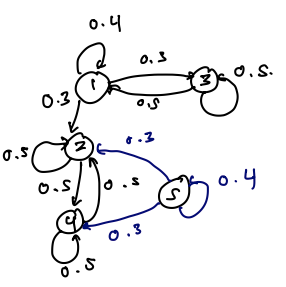
\includegraphics[width=0.5\textwidth]{mc1}
          \caption{Transition Diagram for part (i)}
          \label{fig:mc1}
        \end{figure}

        From the diagram, it is readily deduced that the communication classes are $\{1,3\}, \; \{2,4\}, \; \{5\}$. The relevant properties are listed in Table \ref{tab:mc1}.
        \begin{table}[htbp]
          \centering
          \begin{tabular}{|c|c|c|}
            \hline
            Class & Recurrent? & Closed? \\
            \hline
            $\{1,3\}$ & Yes & No \\
            \hline
            $\{2,4\}$ & Yes & Yes \\
            \hline
            $\{5\}$ & No & No \\
             \hline
          \end{tabular}
          \caption{MC (i) Properties}
          \label{tab:mc1}
        \end{table}

  \item The format will be identitical to the part above. The chain is portrayed in Figure \ref{fig:mc2}.

        \begin{figure}[h]
          \centering
          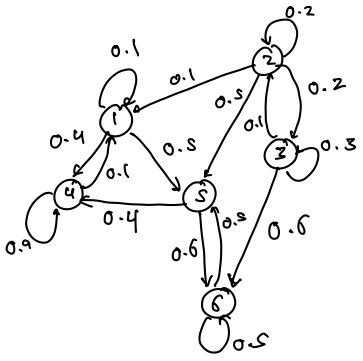
\includegraphics[width=0.5\textwidth]{mc2}
          \caption{Transition Diagram for part (ii)}
          \label{fig:mc2}
        \end{figure}
        The communication classes are $\{1,4,5,6\},\{2,3\}$. The relevant properties are listed in Table \ref{tab:mc2}.

        \begin{table}[htbp]
          \centering
          \begin{tabular}{|c|c|c|}
            \hline
            Class & Recurrent? & Closed? \\
            \hline
            $\{1,4,5,6\}$ & Yes & Yes \\
            \hline
            $\{2,3\}$ & No & No \\
             \hline
          \end{tabular}
          \caption{MC (i) Properties}
          \label{tab:mc2}
        \end{table}

\end{enumerate}


\section{Problem 2}
\label{sec:problem-2}

\begin{enumerate}
  \item From the transition diagram, it is clear that the only paths allowing the chain to hit 6 can be expressed as a series of self-transitions to 0 and taking the transition leading to the recurrence class containing state 6. Let $V_{i,j}$ denote the probability of hitting $j$ starting at $i$. The probability of the chain hitting six conditioned on starting at state 0, $V_{0,6}$, is computed to be:

        \begin{align*}
          V_{0,6} & = \left(1 + \frac{1}{5} + \left(\frac{1}{5}\right)^{2} + \cdots \right) \cdot \frac{1}{5} \\
          & = \left(\frac{1}{1 - 1/5}\right) \cdot \left(\frac{1}{5}\right) \\
          & = \boxed{\frac{1}{4}}
        \end{align*}

  \item We adopt similar reasoning as the part above. We see that the only valid paths are those which cycle between states $1,2$ until eventually transitioning to state $3$ from state $2$. The relevant probability can be evaluated to be:

        \begin{align*}
          V_{1,3} & = \left(1 + \frac{1}{3} + \left(\frac{1}{3}\right)^{2} + \cdots  \right)  \cdot \left(\frac{2}{3}\right) \\
                  & = \left(\frac{1}{1 - 1/3}\right) \cdot \left(\frac{2}{3}\right) \\
          & = \boxed{1}
        \end{align*}

\item
        This portion amounts to simply calculating the expected number of steps to hit 3 starting from 1, which is considered by the following infinite sum:
        \begin{align*}
          \left(\sum_{n=1}^{\infty} \frac{2n}{3^{n-1}} \right)\cdot \left(\frac{2}{3}\right) = \left(\frac{9}{2}    \right) \cdot \left(\frac{2}{3}\right) = \boxed{3}
        \end{align*}
\end{enumerate}

\section{Problem 3}%
\label{sec:problem-3}

\begin{enumerate}
  \item
        \begin{figure}[h]
          \centering
          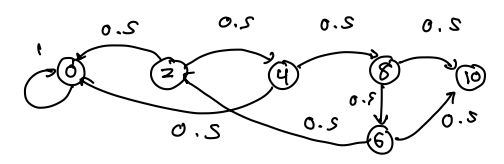
\includegraphics[width=0.7\textwidth]{mc3}
          \caption{Transition Diagram for Gambler's Strategy}
          \label{fig:mc3}
        \end{figure}


        Figure \ref{fig:mc3} depicts the transition diagram for the Markov chain describing the gambler's strategy. The probability $K$ of the gambler eventually winning $\pounds 10$ can be computed by tracing the possible paths to success and accounting for the recurrence:
%
        \begin{align*}
          K = \CondProb{\exists n \geq 0: X_{n} = 10}{X_{0} = 2} & =  \CondProb{2 \rightarrow 4 \rightarrow 8 \rightarrow 10}{X_{0} = 2} \\
                                                             & + \CondProb{2 \rightarrow 4 \rightarrow 6 \rightarrow 8 \rightarrow 10}{X_{0} = 2} \\
                                                             & + \CondProb{2 \rightarrow 4 \rightarrow 8 \rightarrow 6 \rightarrow 2 \rightarrow \cdots}{X_{0} = 2} \\
                                                                 & = \left(\frac{1}{2}\right)^{3} + \left(\frac{1}{2}\right)^{4} + \left(\frac{1}{2}\right)^{4} K
        \end{align*}
        So solving for $K$ shows that $K = 1/5$ as required.

  \item
        As above, the expected value can be expressed through tracing the proper paths and accounting for the recurrence. Let $T_{2}$ be the number of steps the gambler will perform until she either goes bust or succeeds. The average of the r.v is readily computed to be:
        \begin{align*}
          \Exp{T_2} & = 1 \cdot \frac{1}{2}+ 2\cdot \frac{1}{4} + 3 \cdot \frac{1}{8} + 4 \cdot \frac{1}{16} + \left( \Exp{T_2 + 4}\right)\cdot \frac{1}{16} \\
          & = \frac{15}{8} + \frac{1}{16} \Exp{T_2}
        \end{align*}

        Solving for the expected value yields that $\Exp{T_{2}} = 2$.
\end{enumerate}
\section{Problem 4}
\label{sec:problem-4}

Let $Z_{n}$ denote the probability of the Markov chain $(X_n)_{n \geq 0}$ eventually hitting state 0 conditioned on the starting state set to be $n$. The probability we seek is $1 - Z_{1}$. To this end, we begin by first stating the difference equation arising from the transition probabilities of $X$: \[ Z_{n} = p_{n,n+1}\cdot Z_{n+1} + p_{i,i-1}\cdot Z_{i-1} \]


We can solve for the ratio between successive increments of $Z$:
%
\begin{align*}
   Z_{n} & = p_{n,n+1}\cdot Z_{n+1} + p_{i,i-1}\cdot Z_{i-1} \\
  \implies  ( p_{n,n+1} +  p_{n,n-1})\cdot  Z_n  & = p_{n,n+1}\cdot Z_{n+1} + p_{i,i-1}\cdot Z_{i-1} \\
  \implies  p_{i,i+1} \cdot (Z_{{n+1}} - Z_{n})  & = p_{i,i-1} \cdot (Z_n - Z_{{n-1}}) \\
  \implies \frac{Z_{{n+1}} - Z_n}{Z_n - Z_{n-1}} & = \frac{p_{i,i-1}}{p_{i,i+1}} \\
  \implies \frac{Z_{{n+1}} - Z_n}{Z_n - Z_{n-1}} & = \left(\frac{n}{n+1}\right)^{2}
\end{align*}

Let $\gamma_{n} = \frac{Z_{{n+1}} - Z_n}{Z_n - Z_{n-1}}$. It follows that:
\[\frac{Z_{n+1} - Z_{n}}{Z_{1} - Z_{0}} = \prod_{i=1}^{n} \gamma_{i} = \left(\frac{1}{n+1}\right)^{2}\]
and so
\[Z_{n+1} - Z_{n} =  \left(\frac{1}{n+1}\right)^{2}(Z_{1} - 1)\]

by the natural condition that $Z_{0} = 1$. The summing over terms of the left form shows that:

\begin{equation*}
  \label{eq:2}
  \begin{split}
    Z_{n+1} - Z_{1} & = \sum_{i = 1}^n \left(\frac{1}{i+1}\right)^{2} (Z_{1} - 1) \\
    \implies Z_{n+1} & = \left[1 +  \sum_{i = 1}^n \left(\frac{1}{i+1}\right)^{2}\right]Z_{1} -  \sum_{i = 1}^n \left(\frac{1}{i+1}\right)^{2}
  \end{split}
\end{equation*}


The crucial claim is that the sequence $(Z_{n})_{n \geq 0}$ converges to zero as $n \rightarrow \infty$. To see this, recall that $p_{n,n+1} = \left(\frac{n+1}{n}\right)^{2}p_{n,n-1}$. As $n \rightarrow \infty$, the transition probabilities approach $p_{n,n+1} = p_{n,n-1} = \frac{1}{2}$. In other words, the dynamics of the chain converge to that of a symmetric random walk. Hence, for sufficiently large $k$, we may attempt to approximate the distribution of the Markov chain $X$ where $X_{0} = k$ by that of a symmetric random walk. Denote this conditioned chain as $X^{(k)}$. By the Central Limit Theorem and Hajek Page 107, \[\lim_{n \rightarrow \infty}\Prob{\frac{X_{n}^{(k)}}{\sqrt{n}} \leq c} = \Phi(c) \] This implies that sufficiently large $n$ allows us to perform the approximation $X^{(k)}_{n}/\sqrt{n} \sim \standardnormdist$. In particular, $X^{(k)}_{n}$ is tightly concentrated around $k$ in the sense that \[ \lim_{n \rightarrow \infty} \Prob{-\sqrt{cn} \leq X^{(k)}_{n} \leq \sqrt{cn}} = \Phi(c) - \Phi(-c)\]
%
Hence, for sufficiently large $c > 0$ and $n$, $-\sqrt{cn} \leq X_{n}^{(k)} \leq \sqrt{cn}$ with very high probability. As $k \rightarrow \infty$, this will shift this Gaussian to the right. All together, this shows that $Z_{n} \rightarrow 0$ as $n \rightarrow \infty$.

In light of this observation, we can take the limit of both sides of the expression for $Z_{n+1}$ above to yield the required probablity:

\begin{align*}
  0 & = \left[1 +  \sum_{i = 1}^\infty \left(\frac{1}{i+1}\right)^{2}\right]Z_{1} -  \sum_{i = 1}^\infty \left(\frac{1}{i+1}\right)^{2} \\
  \implies Z_{1} & = \frac{\sum_{i=1}^{\infty}\left(\frac{1}{i+1}\right)^{2}}{1 + \sum_{i=1}^{\infty}\left(\frac{1}{i+1}\right)^{2}} \\
  \implies 1 - Z_{1} & = \frac{1}{\sum_{i=0}^{\infty}\left(\frac{1}{i+1}\right)^{2}} \\
 & = \boxed{\frac{6}{\pi^{2}}}
\end{align*}

\section{Problem 5}
\label{sec:problem-5}

Let $X_{n}$ be the number of white balls in urn at the $n^{{th}}$ step. In total, there are three possible evolutions of this process in respect to any fixed state: the number of white, black balls stays the same, a white ball is removed and a black ball is added, and a black ball is removed to be replaced by a white ball. Observe then that these possible states and their transition probabilities only depend on the current number of white, black balls. Thus, this process satisfies the Markov property. As such, its transition probabilities can be determined to be:

\begin{equation*}
P_{ij} = \begin{cases}
           p \cdot \frac{i}{N} + (1-p) \cdot \frac{N-i}{N} & j = i \\
           p \cdot \frac{N-i}{N} & j = i +1 \\
           (1-p)\cdot \frac{i}{N} & j = i -1 \\
           p & i = 0, j=1 \text{ or } i = j = N \\
           1-p & i=N, j = N -1 \text{ or } i = j = 0
         \end{cases}
\end{equation*}


\end{document}
